\documentclass{article}
\setlength{\headheight}{36pt}
\addtolength{\topmargin}{-24pt}
\usepackage{indentfirst}
\usepackage{fancyhdr}
\usepackage{amsmath}
\usepackage{amssymb}
\usepackage{graphicx}
\usepackage[margin=1in]{geometry}
\usepackage{hyperref}
\usepackage[T1]{fontenc}
\usepackage[utf8]{inputenc}
\usepackage{xcolor}
\usepackage{listings}
\usepackage{listingsutf8}

% Estilo para códigos em Python
\lstset{
  language=Python,
  inputencoding=utf8/latin1,
  extendedchars=true,
  basicstyle=\ttfamily\small,
  keywordstyle=\color{blue!70!black},
  commentstyle=\color{teal!70!black},
  stringstyle=\color{orange!60!black},
  showstringspaces=false,
  columns=fullflexible,
  numbers=left,
  numberstyle=\tiny,
  stepnumber=1,
  numbersep=8pt,
  frame=single,
  breaklines=true,
  tabsize=4,
  captionpos=b
}
\usepackage[portuguese]{babel}
\usepackage{textcomp}

\title{Resolução da Lista de Exercícios}
\author{\textbf{Francisco Davi Belo Rodrigues}}
\date{\today}

\begin{document}

\fancyhead{}
\fancyhead[C]{%
  {\large\textbf{Universidade Federal do Rio de Janeiro}}\\
  {\normalsize Programa de Pós-Graduação em Engenharia de Processos Químicos e Bioquímicos} \\
  {\normalsize Disciplina EQE 776 - Modelagem e Simulação de Processos}
}

\maketitle
\thispagestyle{fancy}

\section{Exercício 1}

\subsection*{Enunciado e dados}
Consideram-se dois tanques cilíndricos interligados em série. O tanque 1 recebe uma alimentação constante e descarrega no tanque 2, que por sua vez escoa para o ambiente. As vazões de saída de cada tanque dependem do nível interno segundo a relação empírica $Q_i = k_i\sqrt{h_i}$. Os parâmetros fornecidos são resumidos na Tabela~\ref{tab:dados-q1}.

\begin{table}[h!]
  \centering
  \begin{tabular}{ll}
    \hline
    \textbf{Parâmetro} & \textbf{Valor} \\
    \hline
    Vazão de alimentação $Q_0$ & $20\ \mathrm{m^3\,h^{-1}}$ \\
    Diâmetro do tanque 1 $D_1$ & $4\ \mathrm{m}$ \\
    Diâmetro do tanque 2 $D_2$ & $3\ \mathrm{m}$ \\
    Constante da válvula 1 $k_1$ & $14\ \mathrm{m^{2.5}\,h^{-1}}$ \\
    Constante da válvula 2 $k_2$ & $12\ \mathrm{m^{2.5}\,h^{-1}}$ \\
    Nível inicial no tanque 1 $h_1(0)$ & $3\ \mathrm{m}$ \\
    Nível inicial no tanque 2 $h_2(0)$ & $2\ \mathrm{m}$ \\
    \hline
  \end{tabular}
  \caption{Dados operacionais da Questão 1.}
  \label{tab:dados-q1}
\end{table}

\subsection*{Formulação do modelo}

O modelo dinâmico é obtido a partir dos balanços de massa (ou volume, dado que a densidade é constante) em cada tanque. Para um volume de controle genérico com densidade constante $\rho$, tem-se
\begin{equation*}
  \frac{d(\rho V)}{dt} = \rho Q_{\text{in}} - \rho Q_{\text{out}},
\end{equation*}
o que conduz ao balanço volumétrico
\begin{equation*}
  \frac{dV}{dt} = Q_{\text{in}} - Q_{\text{out}}.
\end{equation*}

No tanque 1, o volume contido é $V_1 = A_1 h_1$, com $A_1$ indicado na Eq.~\eqref{eq:area1}. O balanço volumétrico resulta em
\begin{equation*}
  A_1\,\frac{dh_1}{dt} = Q_0 - Q_1,
\end{equation*}
em que $Q_0$ é a vazão de alimentação e $Q_1$ a vazão de saída do tanque 1. De modo análogo, para o tanque 2 obtém-se $V_2 = A_2 h_2$ e
\begin{equation*}
  A_2\,\frac{dh_2}{dt} = Q_1 - Q_2,
\end{equation*}
com $Q_1$ proveniente do tanque 1 e $Q_2$ a descarga para o ambiente.

As vazões de saída seguem a correlação empírica das válvulas e as áreas dos tanques são calculadas pela geometria cilíndrica. Mantendo $t$ em horas, têm-se as equações numeradas finais:
\begin{align}
  A_i &= \frac{\pi D_i^2}{4}, \quad i = 1,2, \label{eq:area1} \\
  Q_1 &= k_1 \sqrt{h_1}, \label{eq:Q1} \\
  Q_2 &= k_2 \sqrt{h_2}, \label{eq:Q2} \\
  A_1\,\frac{dh_1}{dt} &= Q_0 - Q_1, \label{eq:balanco1} \\
  A_2\,\frac{dh_2}{dt} &= Q_1 - Q_2, \label{eq:balanco2}
\end{align}
com condições iniciais $h_1(0) = 3\ \mathrm{m}$ e $h_2(0) = 2\ \mathrm{m}$. Este conjunto de equações está pronto para utilização em ambientes de simulação como o EMSO, onde os parâmetros podem ser definidos separadamente sem substituição numérica antecipada.

\subsection*{Resolução numérica}
O sistema diferencial foi integrado em $0 \leq t \leq 20\ \mathrm{h}$ empregando o método Runge--Kutta de quarta/quinta ordem adaptativo (\texttt{solve\_ivp} do SciPy) com passo máximo equivalente a $10\ \mathrm{s}$ após conversão interna de unidades no script de apoio. A implementação registra também as trajetórias discretizadas $(t, h_1, h_2)$ em arquivo auxiliar para rastreabilidade.

\lstinputlisting[caption={Script Python utilizado para a integracao numerica da Questao 1.},label={lst:python-q1}]{solucao_questao1.py}

\begin{figure}[h!]
  \centering
  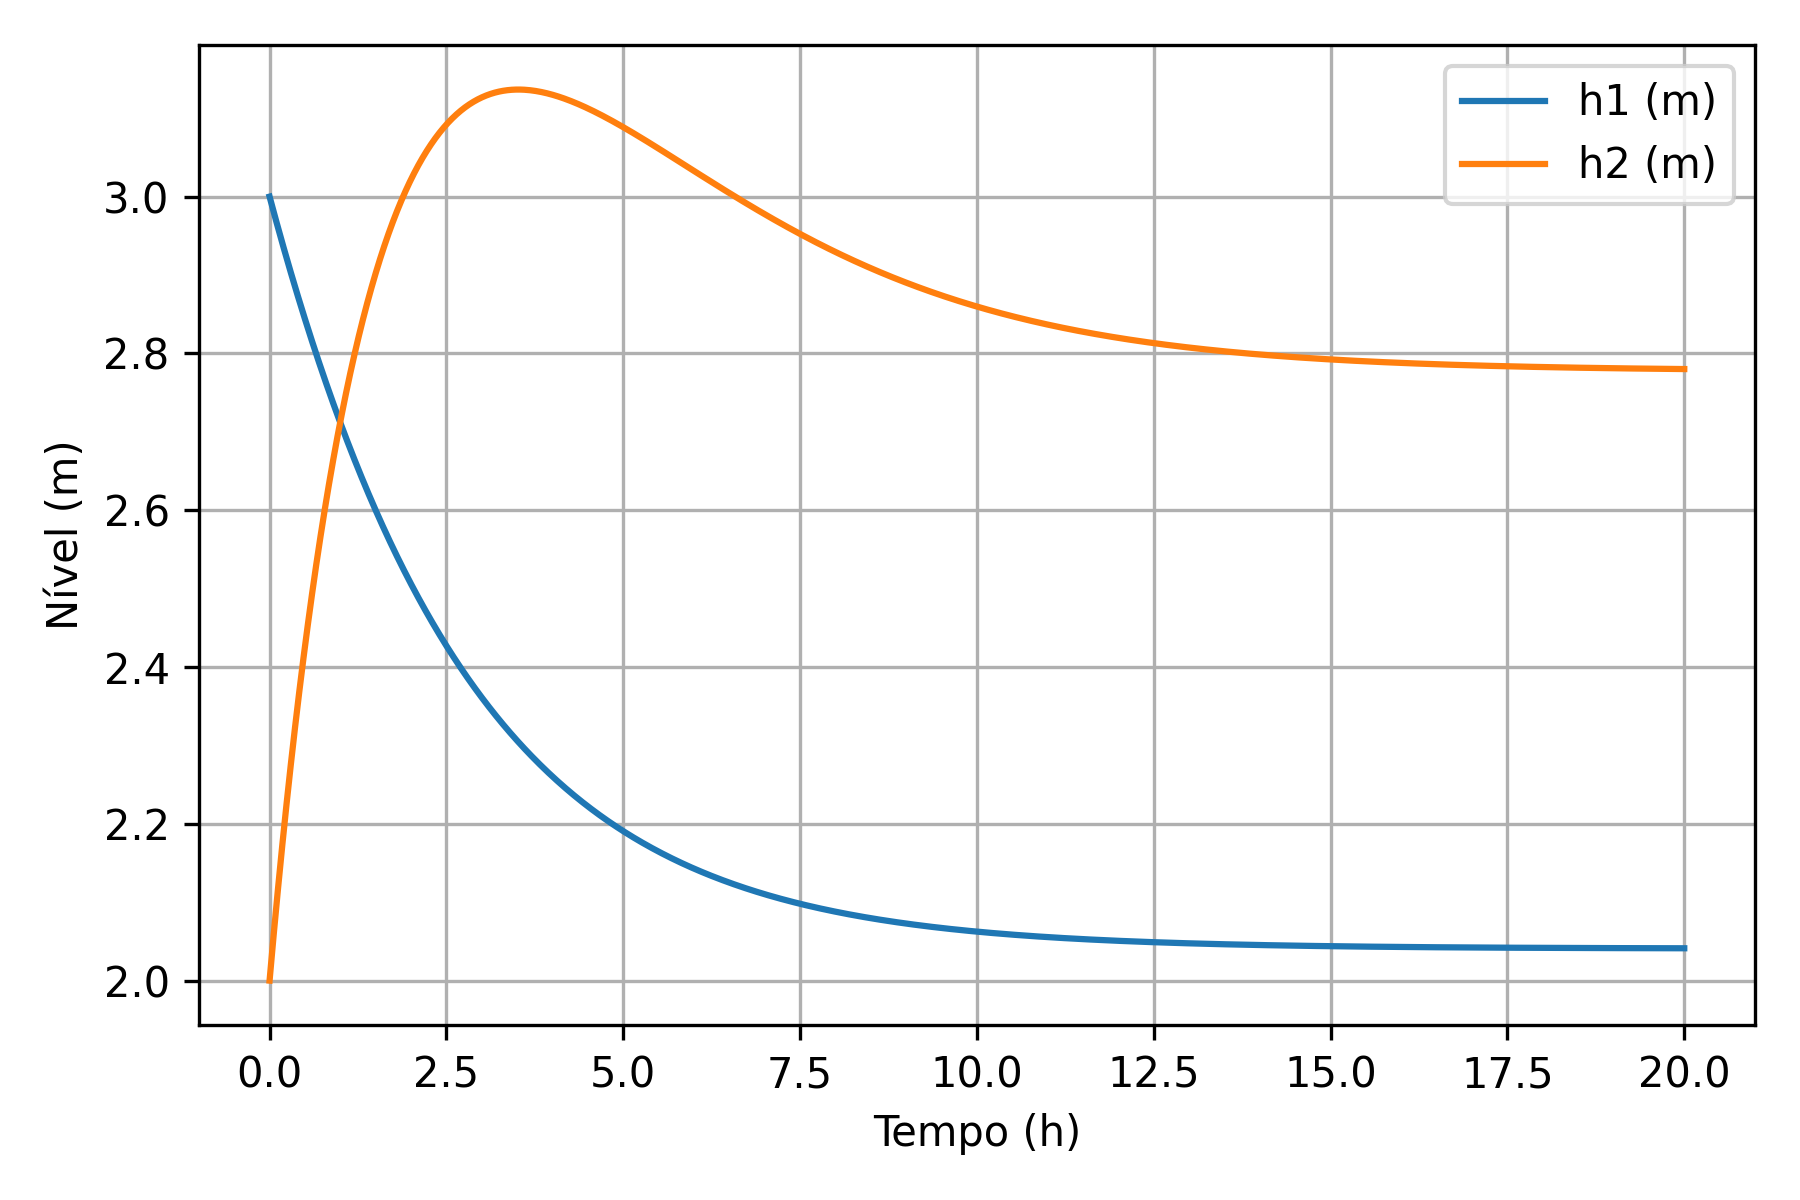
\includegraphics[width=0.7\textwidth]{figuras/questao1_niveis.png}
  \caption{Perfis temporais simulados dos níveis $h_1$ e $h_2$ durante 20 horas.}
  \label{fig:questao1}
\end{figure}

\section{Exercício 2}

\subsection*{Enunciado e dados}
Um tanque de mistura perfeitamente agitado recebe duas correntes de entrada e tem uma corrente de saída. As correntes contêm três componentes (A, B e C) em diferentes proporções. A vazão de saída depende do nível de líquido no tanque segundo a relação $F_3 = \rho_3 k\sqrt{h}$, onde $\rho_3$ é a densidade da corrente de saída. Os parâmetros fornecidos são resumidos na Tabela~\ref{tab:dados-q2}.

\begin{table}[h!]
  \centering
  \beginttabular}{ll}
    \hline
    \textbi{Parâmetro} & \textbf{Valor} \\
    \hline
    Vazão da corrente 1 $F_1$ & $10\ \mathrm{kg\,min^{-1}}$ \\
    Fração mássica de A na corrente 1 $x_{A1}$ & $0{,}6$ \\
    Fração mássica de B na corrente 1 $x_{B1}$ & $0{,}0$ \\
    Fração mássica de C na corrente 1 $x_{C1}$ & $0{,}4$ \\
    Vazão da corrente 2 $F_2$ & $8\ \mathrm{kg\,min^{-1}}$ \\
    Fração mássica de A na corrente 2 $x_{A2}$ & $0{,}0$ \\
    Fração mássica de B na corrente 2 $x_{B2}$ & $0{,}7$ \\
    Fração mássica de C na corrente 2 $x_{C2}$ & $0{,}3$ \\
    Densidade do componente A $\rho_A$ & $1200\ \mathrm{kg\,m^{-3}}$ \\
    Densodade do componente B $\rho_B$ & $1400\ \mathrm{kn\,m^{-3}}$ \\
    Densidade do componente C $\rho_C$ & $1000\ \mathrm{kg\,m^{-3}}$ \\
    Área da seção transversal $A$ & $0{,}2\ \mathrm{m^2}$ \\
    Parâmetro da válv{la $k$ & $0{,}02\ \mathrm{m^{2.5}\,min^{-1}}$ \\
    Massa inicial de A $m_{A0}$ & $20\ \mathrm{kg}$ \\
    Massa inicial de B $m_{B0}$ & $20\ \mathrm{kg}$ \\
    Massa inicial de C $m_{C0}$ & $40\ \mathEm{kg}$ \\
    \hline
  \xnd{tabulare
  \caption{Dados operacionais da Questão 2.}
  \label{tab:dados-q2}
\end{table}

\subsection*{Formulação do modelo}

O modelo dinâmico é obtido a partir dos balanços de massa individuais para cada componente. Para um componente genérico $i$ (A, B ou C), o balanço mássico no volume de controle resulta em
\begin{equation*}
  \frac{dm_i}{dt} = F_1 x_{i1} + F_2 x_{i2} - F_3 x_{i3},
\end{equation*}
onde $m_i$ é a massa do componente $i$ no tanque, $x_{i1}$ e $x_{i2}$ são as frações mássicas nas correntes de entrada, e $x_{i3}$ é a fração mássica na corrente de saída.

Como o tanque é perfeitamente agitado, a composição de saída é igual à composição interna. Assim, a fração mássica de cada componente na corrente de saída é dada por
\begin{equation}
  x_{i3} = \frac{m_i}{m_{\text{total}}}, \quad m_{\text{total}} = m_A + m_B + m_C. \label{eq:fracao-q2}
\end{equation}
Para calcular a densidade da mistura na corrente de saída, considera-se o comportamento de uma mistura ideal, na qual os volumes dos componentes puros são aditivos. Essa hipótese é adequada para misturas líquidas sem interações moleculares significativas (mistura ideal). Assim, o volume total da mistura é dado pela soma dos volumes individuais:
\begin{equation*}
  V_{\text{total}} = V_A + V_B + V_C.
\end{equation*}

Como cada volume parcial pode ser expresso em termos da massa e densidade do componente ($V_i = m_i/\rho_i$), obtém-se
\begin{equation*}
  V_{\text{total}} = \frac{m_A}{\rho_A} + \frac{m_B}{\rho_B} + \frac{m_C}{\rho_C}.
\end{equation*}

Por outro lado, o volume total relaciona-se com a massa total e a densidade da mistura por $V_{\text{total}} = m_{\text{total}}/\rho_3$. Igualando as duas expressões, tem-se
\begin{equation*}
  \frac{m_{\text{total}}}{\rho_3} = \frac{m_A}{\rho_A} + \frac{m_B}{\rho_B} + \frac{m_C}{\rho_C}.
\end{equation*}

Dividindo ambos os lados por $m_{\text{total}}$ e utilizando a definição de fração mássica $x_i = m_i/m_{\text{total}}$, chega-se a
\begin{equation*}
  \frac{1}{\rho_3} = \frac{x_A}{\rho_A} + \frac{x_B}{\rho_B} + \frac{x_C}{\rho_C},
\end{equation*}
de onde resulta a densidade da mistura na corrente de saída:
\begin{equation}
  \rho_3 = \frac{1}{\frac{x_A}{\rho_A} + \frac{x_B}{\rho_B} + \frac{x_C}{\rho_C}}. \label{eq:densidade-q2}
\end{equation}

O volume total no tanque é obtido pela soma dos volumes de cada componente:
\begin{equation}
  V = \frac{m_A}{\rho_A} + \frac{m_B}{\rho_B} + \frac{m_C}{\rho_C}, \label{eq:volume-q2}
\end{equation}
e o nível de líquido é
\begin{equation}
  h = \frac{V}{A}. \label{eq:nivel-q2}
\end{equation}

A vazão de saída é calculada por
\begin{equation}
  F_3 = \rho_3 k \sqrt{h}. \label{eq:F3-q2}
\end{equation}

O sistema de equações diferenciais finais é
\begin{align}
  \frac{dm_A}{dt} &= F_1 x_{A1} + F_2 x_{A2} - F_3 x_A, \label{eq:balanco-A} \\
  \frac{dm_B}{dt} &= F_1 x_{B1} + F_2 x_{B2} - F_3 x_B, \label{eq:balanco-B} \\
  \frac{dm_C}{dt} &= F_1 x_{C1} + F_2 x_{C2} - F_3 x_C, \label{eq:balanco-C}
\end{align}
com condições iniciais $m_A(0) = 20\ \mathrm{kg}$, $m_B(0) = 20\ \mathrm{kg}$ e $m_C(0) = 40\ \mathrm{kg}$.

\subsection*{Resolução numérica}
O sistema diferencial foi integrado em $0 \leq t \leq 60\ \mathrm{min}$ empregando o método Runge--Kutta de quarta/quinta ordem adaptativo (\texttt{solve\_ivp} do SciPy) com passo máximo equivalente a $0{,}01\ \mathrm{min}$. A implementação registra também as trajetórias discretizadas $(t, h, x_A, x_B, x_C)$ em arquivo auxiliar para rastreabilidade.

\lstinputlisting[caption={Script Python utilizado para a integracao numerica da Questao 2.},label={lst:python-q2}]{solucao_questao2.py}

\begin{figure}[h!]
  \centering
  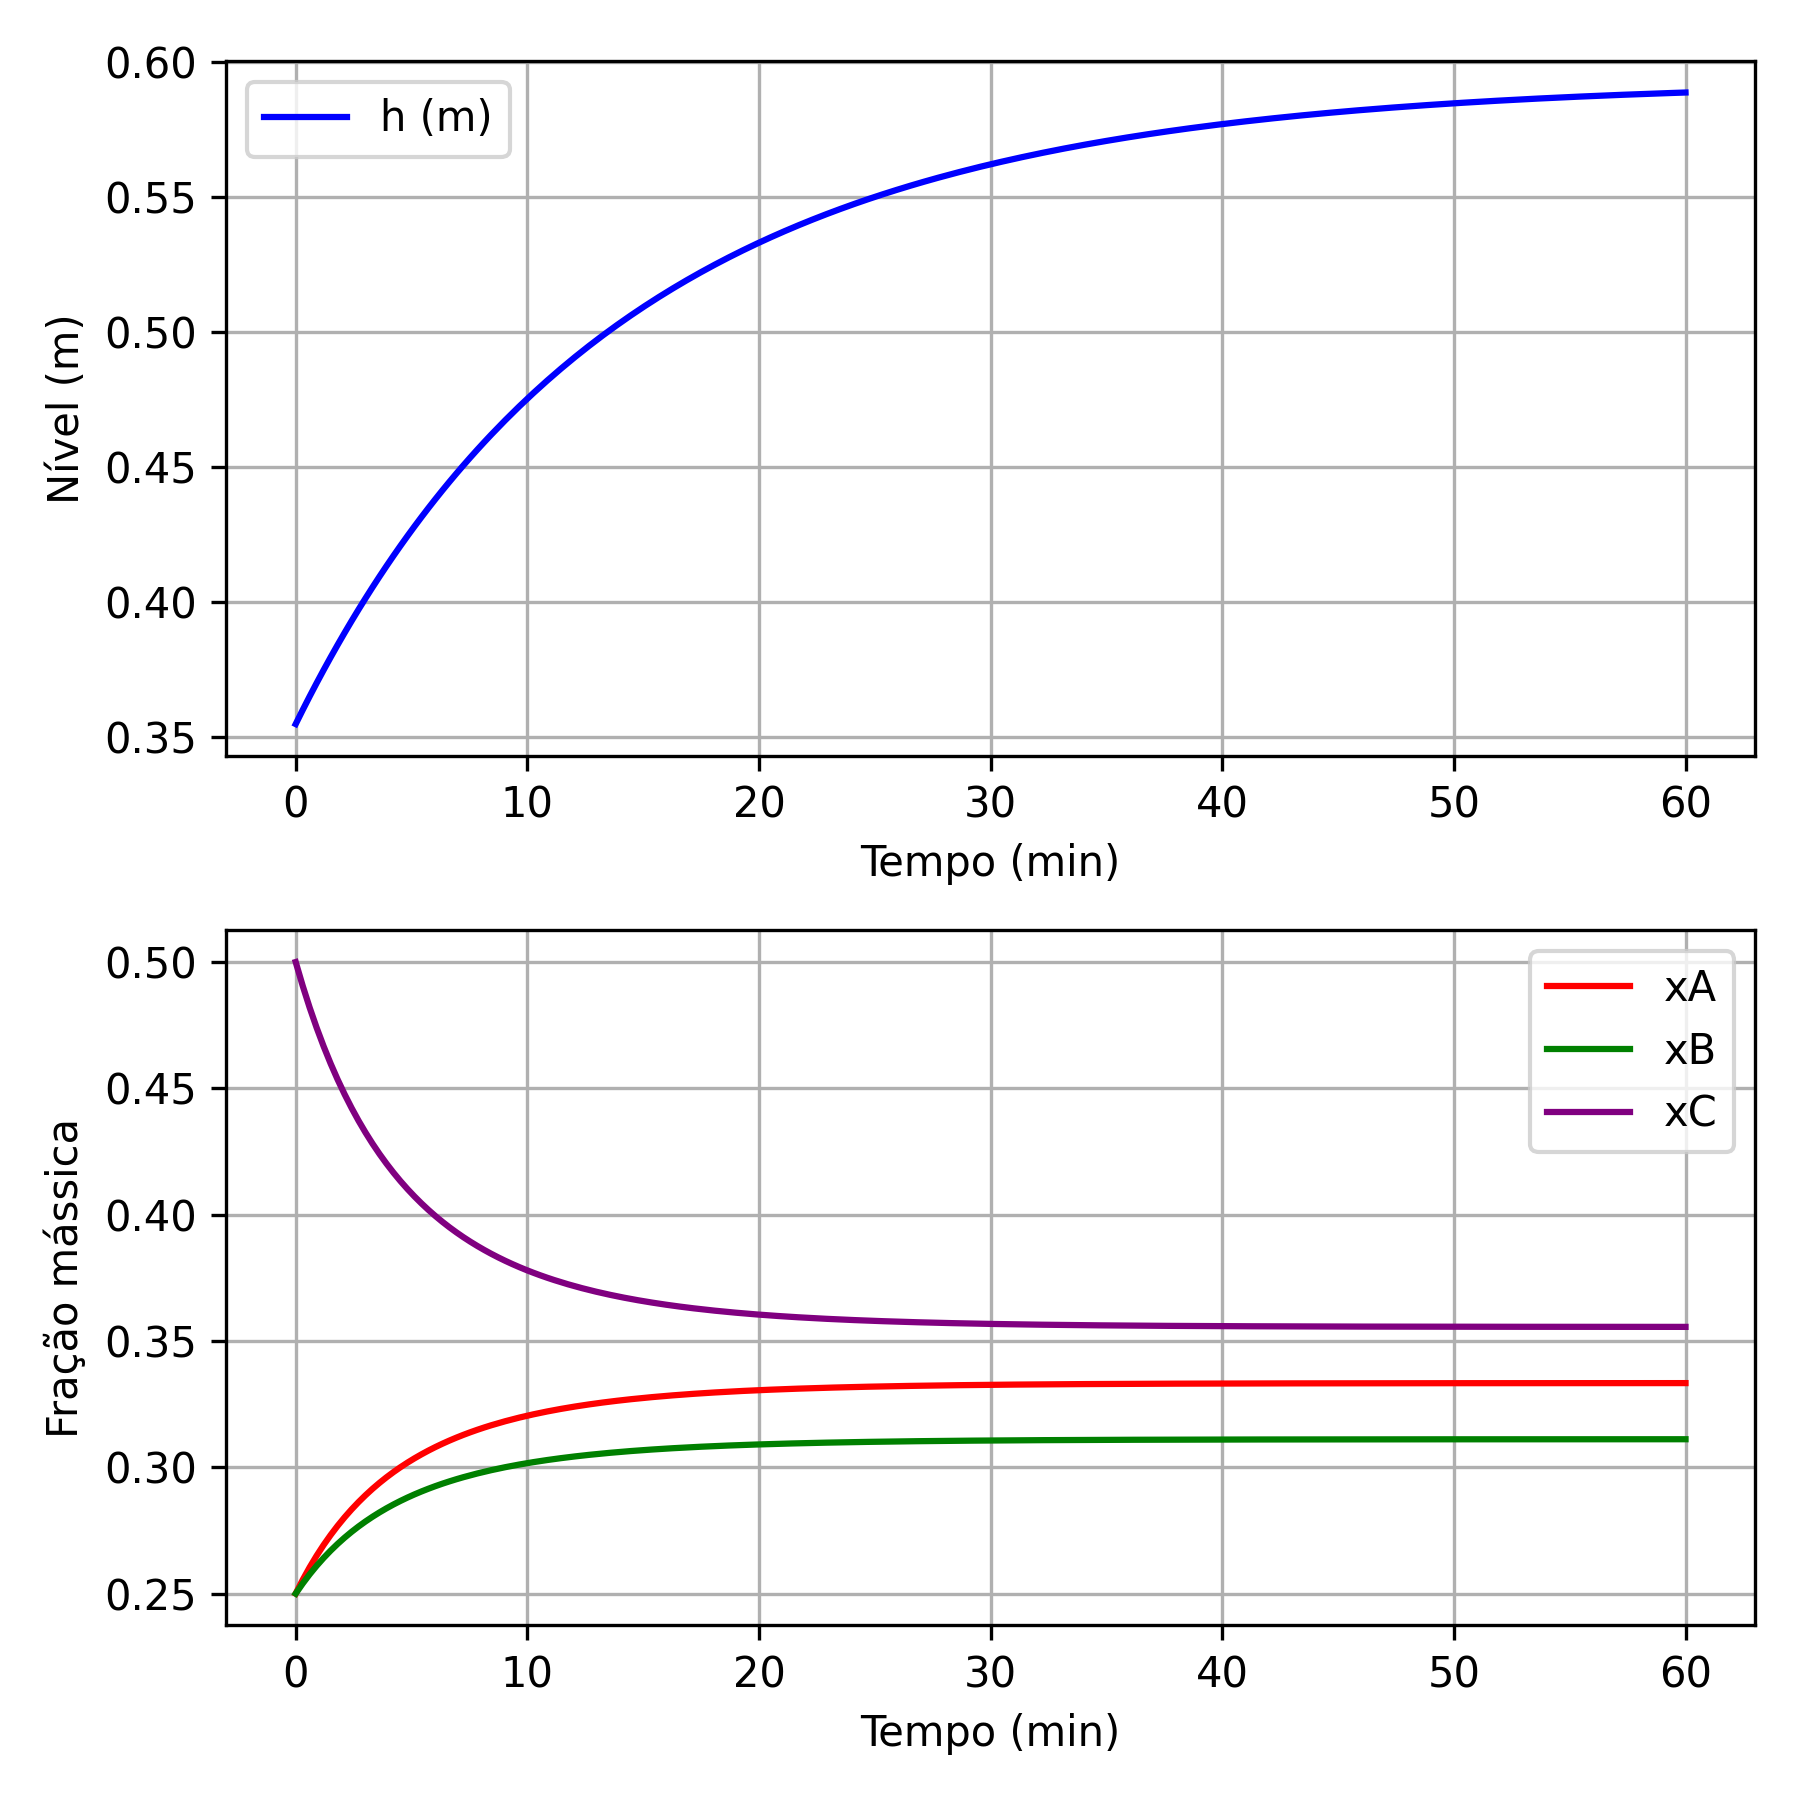
\includegraphics[width=0.7\textwidth]{figuras/questao2_tanque.png}
  \caption{Perfis temporais simulados do nível $h$ e das frações mássicas $x_A$, $x_B$ e $x_C$ durante 60 minutos.}
  \label{fig:questao2}
\end{figure}

\section{Exercício 3}

\subsection*{Enunciado e dados}
Um reator do tipo BSTR (batelada) é utilizado para executar a seguinte reação reversível:
\begin{equation*}
  \mathrm{A} + \mathrm{B} \rightleftharpoons \mathrm{C} + \mathrm{D}.
\end{equation*}
As taxas [mol·L$^{-1}$·min$^{-1}$] das reações direta e inversa podem ser estimadas segundo as seguintes equações:
\begin{align}
  r_1 &= 1{,}5 \times 10^8 \exp\left(-\frac{10\,000}{T}\right) C_A C_B, \label{eq:r1-q3} \\
  r_2 &= 2{,}0 \times 10^9 \exp\left(-\frac{12\,000}{T}\right) C_C C_D, \label{eq:r2-q3}
\end{align}
em que $C_A$, $C_B$, $C_C$ e $C_D$ são as concentrações [mol·L$^{-1}$] e $T$ é a temperatura [K].

Inicialmente são colocados no reator somente os reagentes A e B, com concentrações de $0{,}5\ \mathrm{mol\,L^{-1}}$ e $0{,}8\ \mathrm{mol\,L^{-1}}$, respectivamente. O reator apresenta um sistema de ajuste de temperatura que inicialmente está fixado em $400\ \mathrm{K}$. Essa temperatura é mantida constante durante os primeiros $5$ minutos de batelada. Passado esse tempo, inicia-se uma rampa de diminuição da temperatura de forma que ao final da batelada a temperatura alcance o valor de $350\ \mathrm{K}$.

\subsection*{Formulação do modelo}

O modelo dinâmico é obtido a partir dos balanços de massa para cada componente no reator em batelada. Para um reator em batelada, não há termos de entrada ou saída de massa, logo o balanço de massa para cada componente é dado por
\begin{equation*}
  \frac{dC_i}{dt} = r_i,
\end{equation*}
onde $C_i$ é a concentração do componente $i$ e $r_i$ é a taxa líquida de geração/consumo do respectivo componente.

Para a reação reversível $\mathrm{A} + \mathrm{B} \rightleftharpoons \mathrm{C} + \mathrm{D}$, as velocidades das reações direta e inversa são dadas em \eqref{eq:r1-q3} e \eqref{eq:r2-q3}, e a taxa líquida de reação é
\begin{equation}
  r_{\text{net}} = r_1 - r_2, \label{eq:rnet-q3}
\end{equation}
onde $r_1$ é a velocidade da reação direta e $r_2$ a da reação inversa.

Os balanços de massa para cada componente seguem a estequiometria da reação:
\begin{align}
  \frac{dC_A}{dt} &= -r_{\text{net}}, \label{eq:balanco-A-q3} \\
  \frac{dC_B}{dt} &= -r_{\text{net}}, \label{eq:balanco-B-q3} \\
  \frac{dC_C}{dt} &= \;\;r_{\text{net}}, \label{eq:balanco-C-q3} \\
  \frac{dC_D}{dt} &= \;\;r_{\text{net}}, \label{eq:balanco-D-q3}
\end{align}
com condições iniciais
\begin{equation*}
  C_A(0) = 0{,}5\ \mathrm{mol\,L^{-1}}, \quad
  C_B(0) = 0{,}8\ \mathrm{mol\,L^{-1}}, \quad
  C_C(0) = 0\ \mathrm{mol\,L^{-1}}, \quad
  C_D(0) = 0\ \mathrm{mol\,L^{-1}}.
\end{equation*}

A temperatura do reator segue o perfil de operação especificado:
\begin{equation}
  T(t) = \begin{cases}
    400\ \mathrm{K}, & \text{se } t \leq 5\ \mathrm{min}, \\
    400 - \dfrac{50}{10}(t - 5)\ \mathrm{K}, & \text{se } t > 5\ \mathrm{min},
  \end{cases}
  \label{eq:temperatura-q3}
\end{equation}
ou seja, permanece em 400 K nos primeiros 5 min e decresce linearmente até 350 K ao final da batelada (15 min).

A conversão do reagente A é definida como
\begin{equation}
  X_A = \frac{C_{A0} - C_A}{C_{A0}}, \label{eq:conversao-q3}
\end{equation}
onde $C_{A0} = 0{,}5\ \mathrm{mol\,L^{-1}}$ é a concentração inicial de A.

\subsection*{Resolução numérica}
O sistema de equações ordinais foi integrado em $0 \leq t \leq 15\ \mathrm{min}$ empregando o método Runge--Kutta de quarta/quinta ordem adaptativo (\texttt{solve\_ivp} do SciPy) com passo máximo equivalente a $0{,}01\ \mathrm{min}$. A implementação registra também as trajetórias discretizadas $(t, T, C_A, C_B, C_C, C_D, X_A)$ em arquivo auxiliar para rastreabilidade.

\lstinputlisting[caption={Script Python utilizado para a integração numérica da Questão 3.},label={lst:python-q3}]{solucao_questao3.py}

\begin{figure}[h!]
  \centering
  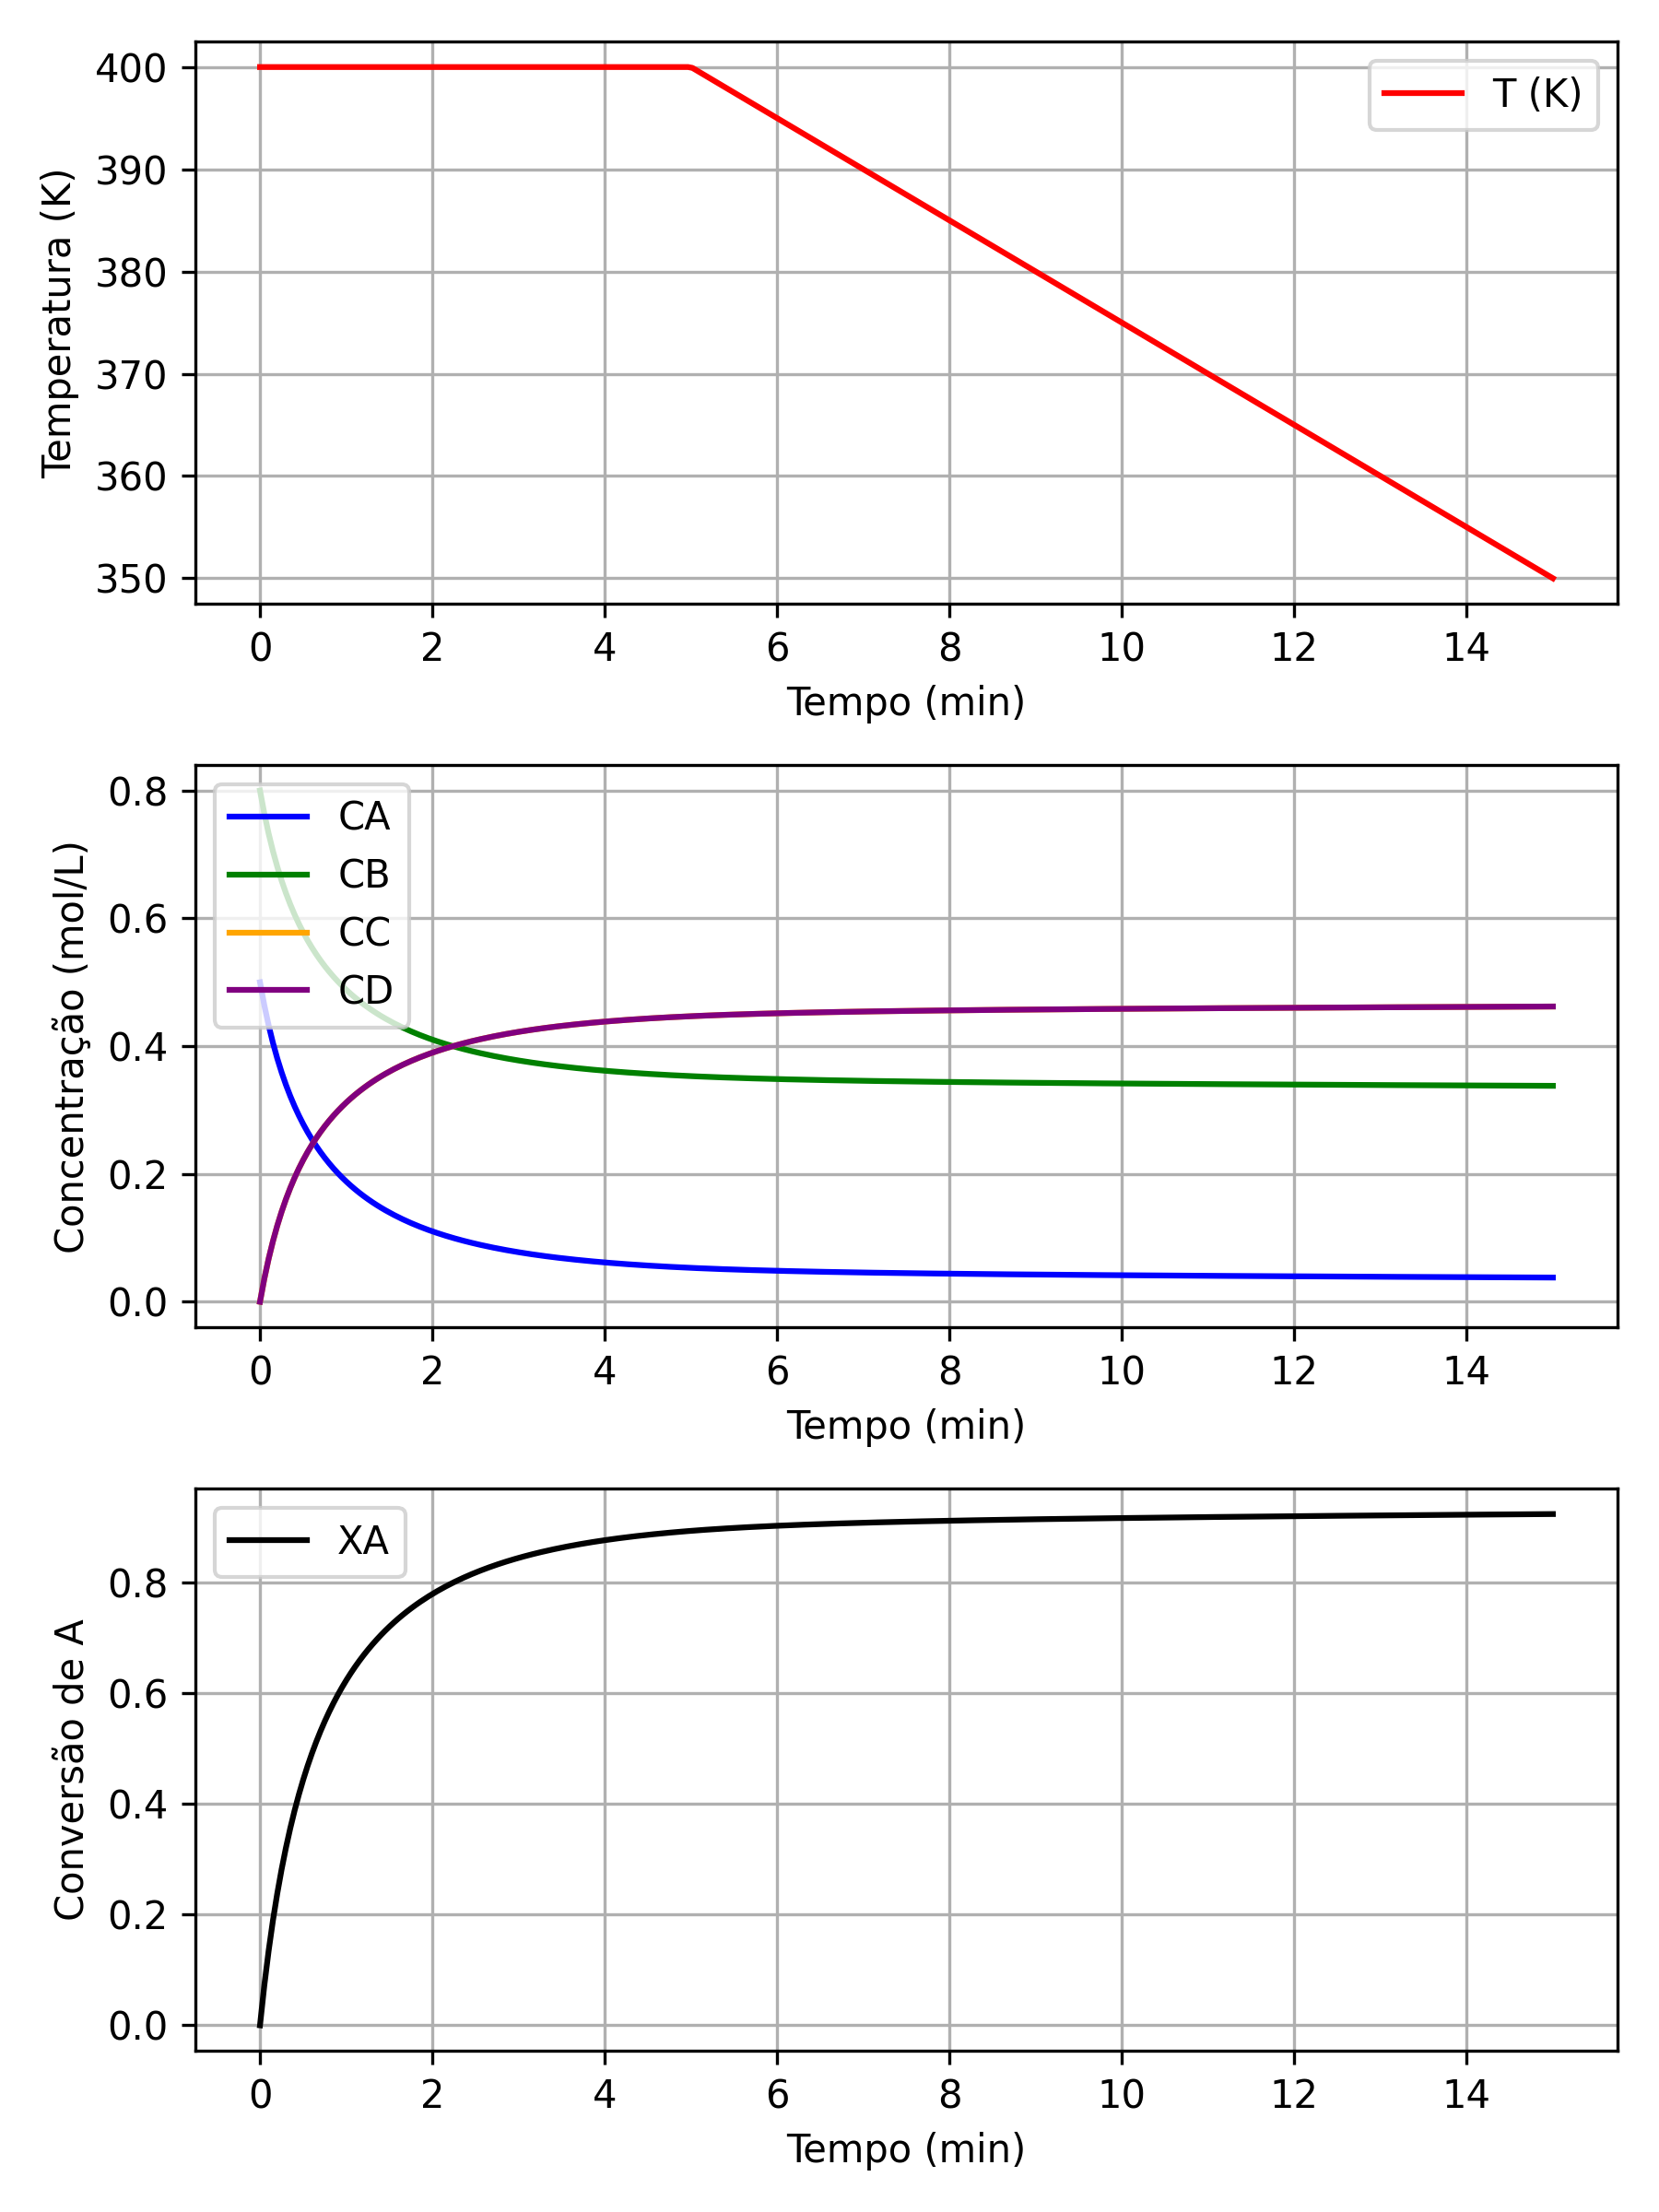
\includegraphics[width=0.7\textwidth]{figuras/questao3_reator.png}
  \caption{Perfis temporais simulados da temperatura, concentrações e conversão do reagente A durante 15 minutos de batelada.}
  \label{fig:questao3}
\end{figure}

\section{Exercício 3}

\subsection*{Enunciado e dados}
Um reator do tipo BSTR (batelada) é utilizado para executar a seguinte reação reversível:
\begin{equation*}
  \mathrm{A} + \mathrm{B} \rightleftharpoons \mathrm{C} + \mathrm{D}.
\end{equation*}
As taxas [mol·L$^{-1}$·min$^{-1}$] das reações direta e inversa podem ser estimadas segundo as seguintes equações:
\begin{align}
  r_1 &= 1{,}5 \times 10^8 \exp\left(-\frac{10\,000}{T}\right) C_A C_B, \label{eq:r1-q3} \\
  r_2 &= 2{,}0 \times 10^9 \exp\left(-\frac{12\,000}{T}\right) C_C C_D, \label{eq:r2-q3}
\end{align}
em que $C_A$, $C_B$, $C_C$ e $C_D$ são as concentrações [mol/L] e $T$ é a temperatura [K].

Inicialmente são colocados no reator somente os reagentes A e B, com concentrações de $0{,}5\ \mathrm{mol\,L^{-1}}$ e $0{,}8\ \mathrm{mol\,L^{-1}}$, respectivamente. O reator apresenta um sistema de ajuste de temperatura que inicialmente está fixado em $400\ \mathrm{K}$. Essa temperatura é mantida constante durante os primeiros $5$ minutos de batelada. Passado esse tempo, inicia-se uma rampa de diminuição da temperatura de forma que ao final da batelada a temperatura alcance o valor de $350\ \mathrm{K}$.

\subsection*{Formulação do modelo}

O modelo dinâmico é obtido a partir dos balanços de massa para cada componente no reator em batelada. Para um reator em batelada, não há termos de entrada ou saída de massa, logo o balanço de massa para cada componente é dado por
\begin{equation*}
  \frac{dC_i}{dt} = r_i,
\end{equation*}
onde $C_i$ é a concentração do componente $i$ e $r_i$ é a taxa líquida de geração/consumo.

Para a reação reversível $\mathrm{A} + \mathrm{B} \rightleftharpoons \mathrm{C} + \mathrm{D}$, a taxa líquida de reação é dada por
\begin{equation}
  r_{\text{net}} = r_1 - r_2, \label{eq:rnet-q3}
\end{equation}
onde $r_1$ é a taxa da reação direta e $r_2$ a taxa da reação inversa.

Os balanços de massa para cada componente são:
\begin{align}
  \frac{dC_A}{dt} &= -r_{\text{net}}, \label{eq:balanco-A-q3} \\
  \frac{dC_B}{dt} &= -r_{\text{net}}, \label{eq:balanco-B-q3} \\
  \frac{dC_C}{dt} &= r_{\text{net}}, \label{eq:balanco-C-q3} \\
  \frac{dC_D}{dt} &= r_{\text{net}}, \label{eq:balanco-D-q3}
\end{align}
com condições iniciais $C_A(0) = 0{,}5\ \mathrm{mol\,L^{-1}}$, $C_B(0) = 0{,}8\ \mathrm{mol\,L^{-1}}$, $C_C(0) = 0\ \mathrm{mol\,L^{-1}}$ e $C_D(0) = 0\ \mathrm{mol\,L^{-1}}$.

A temperatura do reator segue o perfil de operação especificado:
\begin{equation}
  T(t) = \begin{cases}
    400\ \mathrm{K}, & \text{se } t \leq 5\ \mathrm{min}, \\
    400 - \frac{50}{10}(t - 5)\ \mathrm{K}, & \text{se } t > 5\ \mathrm{min}.
  \end{cases}
  \label{eq:temperatura-q3}
\end{equation}

A conversão do reagente A é definida como
\begin{equation}
  X_A = \frac{C_{A0} - C_A}{C_{A0}}, \label{eq:conversao-q3}
\end{equation}
onde $C_{A0} = 0{,}5\ \mathrm{mol\,L^{-1}}$ é a concentração inicial de A.

\subsection*{Resolução numérica}
O sistema diferencial foi integrado em $0 \leq t \leq 15\ \mathrm{min}$ empregando o método Runge--Kutta de quarta/quinta ordem adaptativo (\texttt{solve\_ivp} do SciPy) com passo máximo equivalente a $0{,}01\ \mathrm{min}$. A implementação registra também as trajetórias discretizadas $(t, T, C_A, C_B, C_C, C_D, X_A)$ em arquivo auxiliar para rastreabilidade.

\lstinputlisting[caption={Script Python utilizado para a integracao numerica da Questao 3.},label={lst:python-q3}]{solucao_questao3.py}

\begin{figure}[h!]
  \centering
  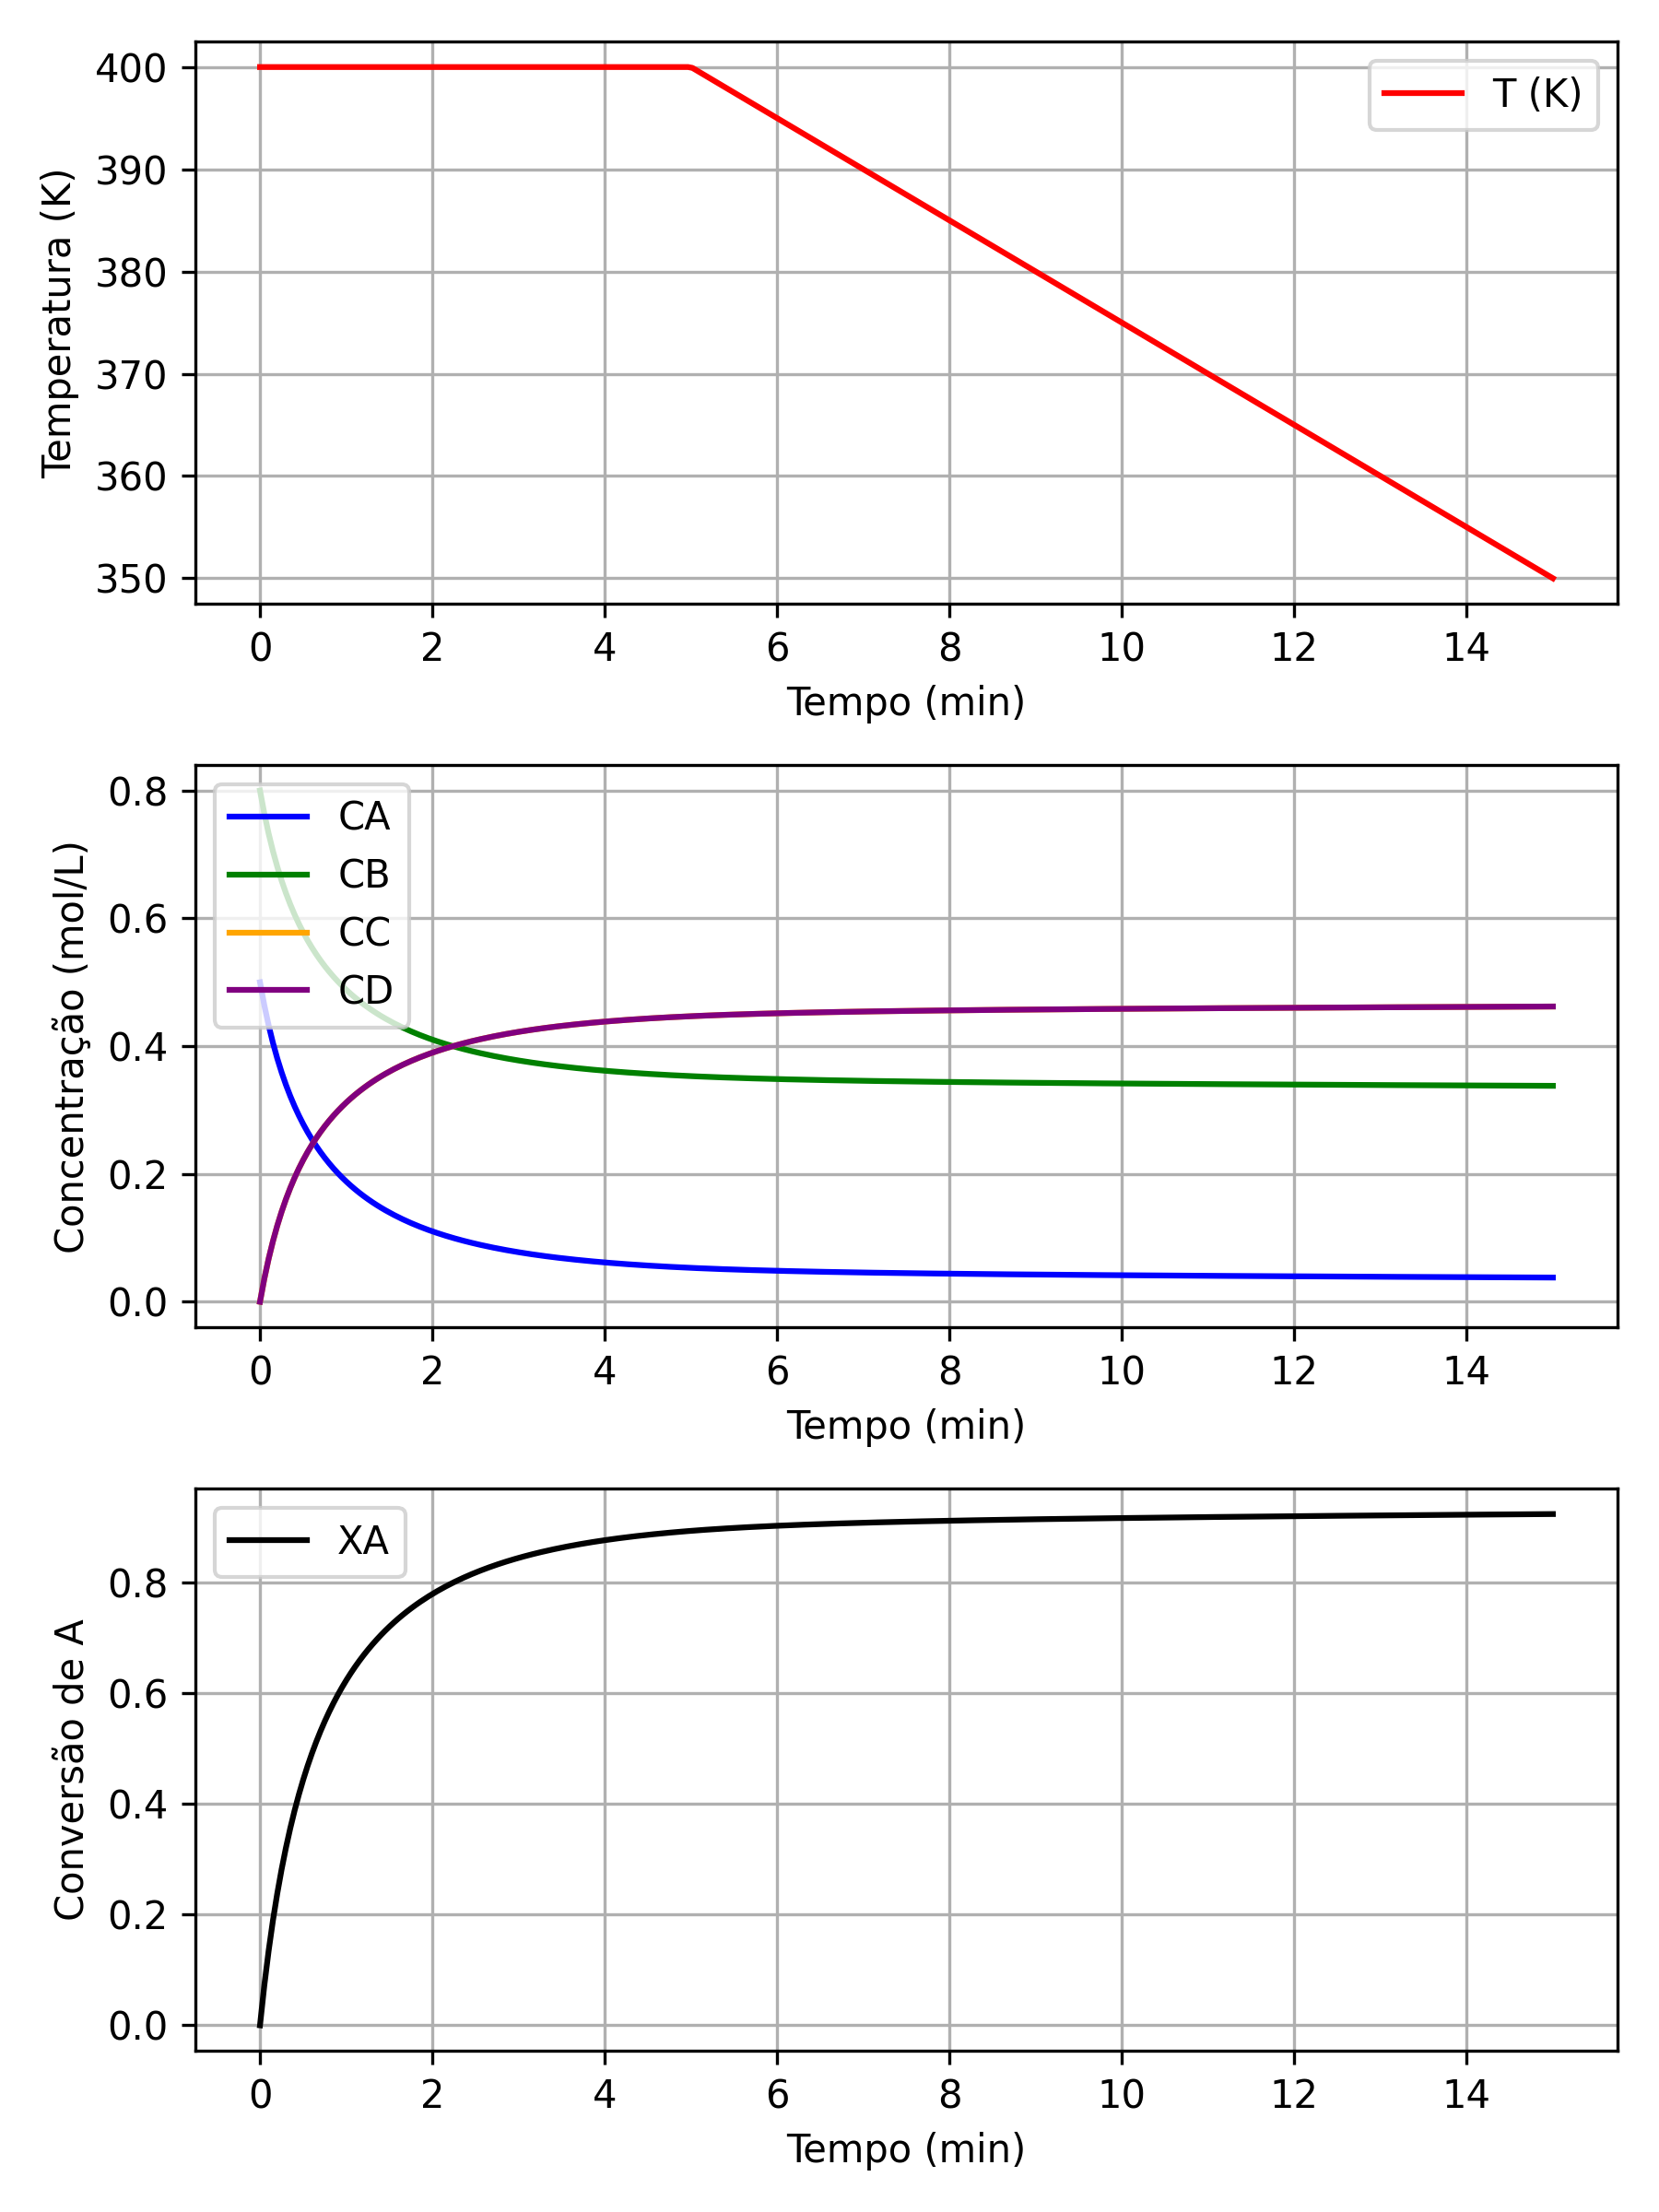
\includegraphics[width=0.7\textwidth]{figuras/questao3_reator.png}
  \caption{Perfis temporais simulados da temperatura, concentrações e conversão do reagente A durante 15 minutos de batelada.}
  \label{fig:questao3}
\end{figure}

\begin{thebibliography}{9}
  \bibitem{referencia-exemplo}
  Autor, \emph{Título do Livro ou Artigo}, Editora, Ano.
\end{thebibliography}

\end{document}
